

\msection{Estimation Under Physical Constraints (Aim 4)}
\vskip-10pt
\background{}
As we have discussed, traditional statistical methods and theory
are oriented toward constraints on properties
such as smoothness.  The
statistical, machine learning, and signal processing communities have
more recently invested heavily 
in notions such as sparsity, manifold structure, and low rank
assumptions.   On the other hand,
classical applied mathematics was driven
by physical problems that can be tightly modeled by PDEs reflecting the underlying
physical laws.  A large gap remains between these traditions.
In particular, we have only the most rudimentary understanding
of how to combine physical models with data driven approaches.

Indeed, this is precisely the perspective of Andrew Majda,
one of the leaders of classical PDE approaches. As
expressed in \cite{majda:12}, 
\begin{quote}
A central issue in contemporary
science is the development of data driven statistical-dynamical models
for times series of a partial subset of observed values 
$u_I(t)\in\reals^{N_1}$, which arise from observations
of nature or from an extremely complex physical model [$\ldots$]
purely data driven ad-hoc regression models are developed through
various criteria to fit the data but by design, do not respect the
underlying
physical dynamics of the partially observed system or the causal
processes
in the dynamics.
\end{quote}
In this paper, Majda and Harlim introduce a family 
of nonlinear regression models.  In a simplified
form, the models can be expressed in terms
of the stochastic differential equation
$$ du_t = \left(Lu_t + B(u_t, u_t) + f_t\right)dt + \sigma dW_t$$
where $u_t\in\reals^N$ and $f_t$ is a known forcing
function, and $dW_t$ is the increment of a Brownian motion.
The key assumption is that the quadratic interactions $B(u_t, u_t)$ are
subject to the \textit{physical constraints of conservation of
  energy},
specified by 
\begin{equation}
u_t \cdot B(u_t, u_t) = 0.
\label{coe}
\end{equation}
The conservation of energy constraint \eqref{coe} is the 
distinguishing feature of the model; otherwise it is a
standard quadratic regression model.

\begin{figure}[t]
\begin{center}
\ \vskip-20pt
\begin{tabular}{ll}
\hskip-10pt
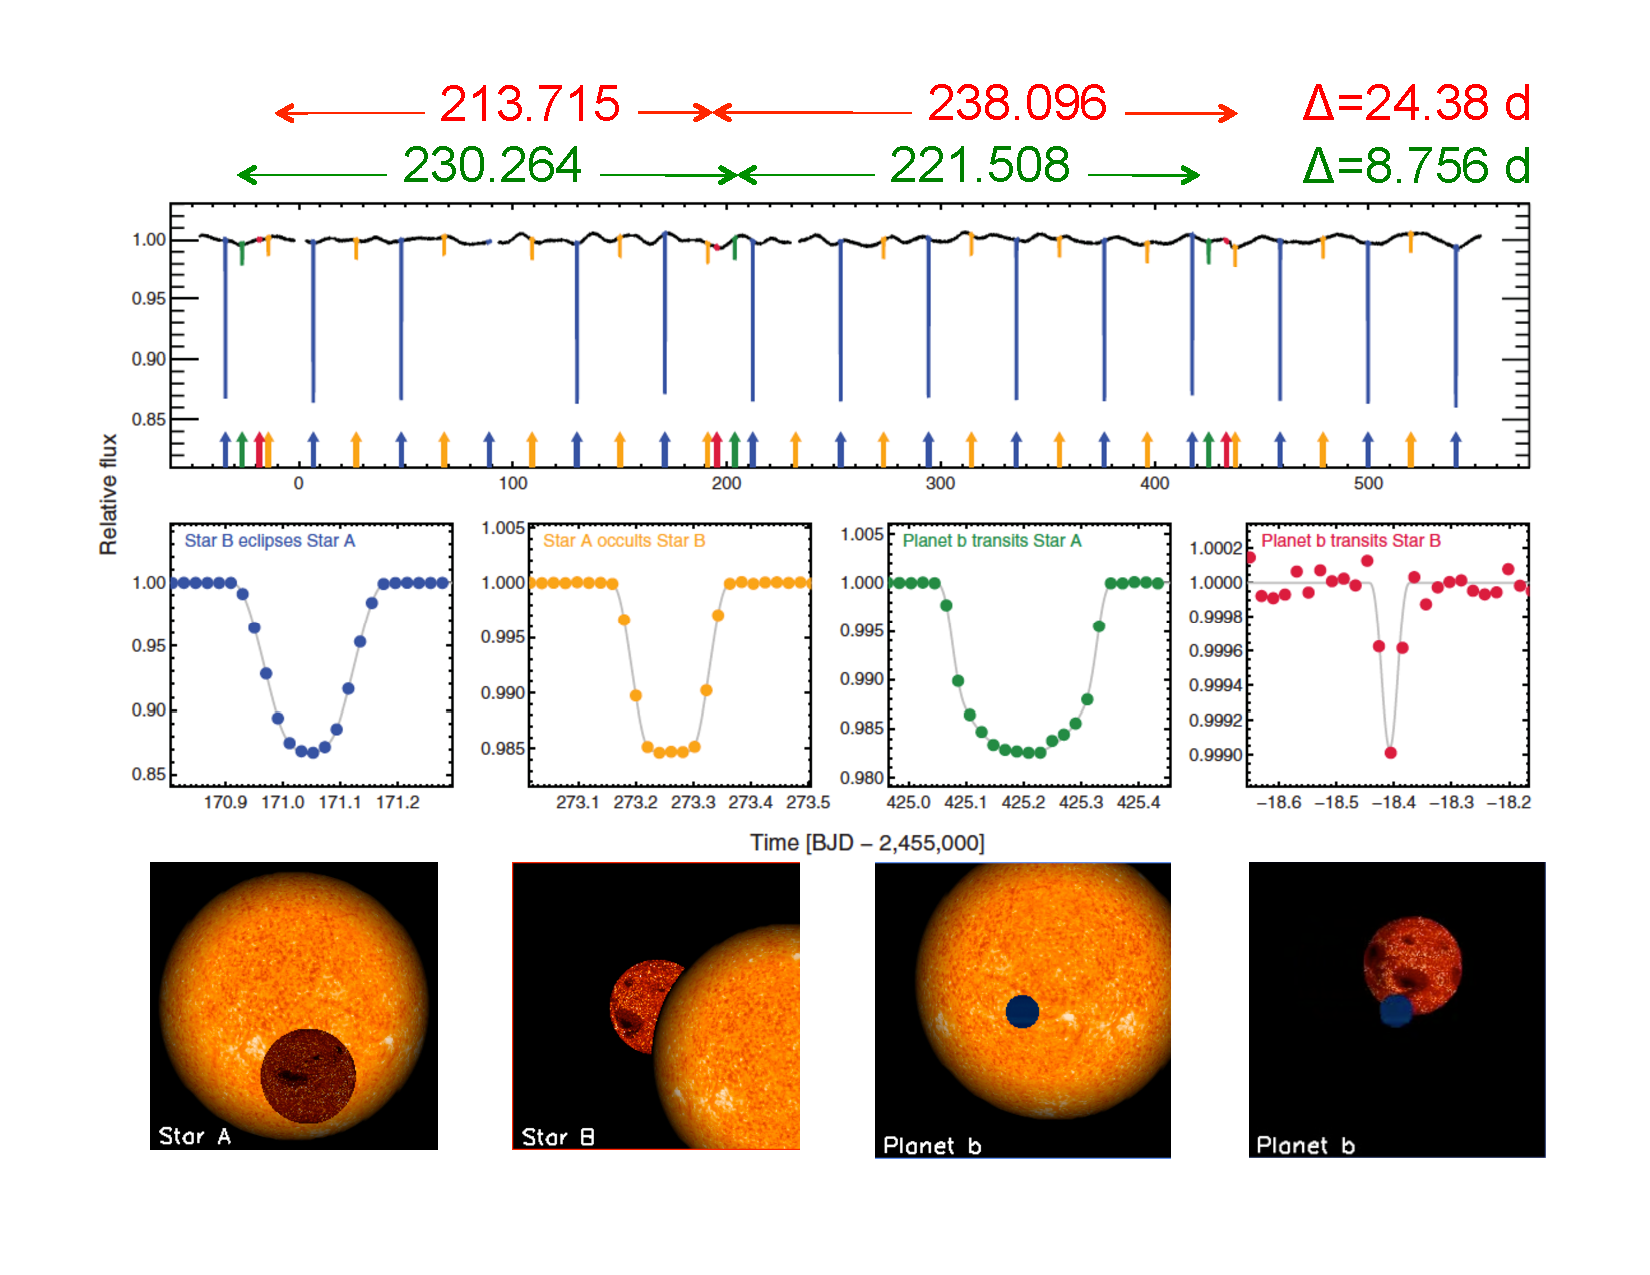
\includegraphics[width=.45\textwidth]{figs/TTV_Fabrycky} \quad & 
\quad \begin{minipage}[b]{2.3in}
\small\linespread{1.0}\selectfont
\stepcounter{figure}
\vskip-15pt
Figure \arabic{figure}. Geometry of planet transits
in a lightcurve from the Kepler data \citep{ttv_fabrycky}.  The
top panel shows the detrended lightcurve, normalized flux.
The transit times for the planet and binary star are shown
as color arrows at the bottom of the panel.  The shape
of planet/binary star transits are different, shown
in the middle panel for the physical configuration shown
in the bottom panel.
\vskip12pt{\ }
\end{minipage}
\label{tradeoff}
\\[-30pt]
\end{tabular}
\end{center}
\end{figure}

As another example of natural physical constraints, let us return to
the problem of detection of exoplanets in lightcurves, considered in
Aim 1. After detrending and computing residuals, the detection problem
can be considered as a sparse normal means testing problem.  Much is
known about optimal testing of sparse normal means or simple geometric
structures \citep{hc:04,DonohoJin:08,huo:06}.  But how can we test for
signals that are governed by known physical laws?  For instance, the
shape of binary star and planet transits is governed by simple
physical and geometrical properties; see Figure~4.

Finally, as another example of statistical modeling
with physical constraints, we mention 
recent work on the long-term goal of building smarter operating
systems under power/performance constraints.
This is joint work with University of Chicago Computer Science Professor
Hank Hoffmann, merging our work in high dimensional
statistics with a computer systems perspective.

The goal is to let the OS  determine how to allocate power among
multiple applications. For example, when running a coupled simulation,
one simulation may be slower than another. Ideally, we would recognize
that these two jobs should run at the same rate, and then shift power
from the faster one to the slower one, reducing overall runtime while
enforcing the power budget.  The required nonlinear optimization is
difficult, as different jobs and even processes within a job will have
different resource needs and different power/performance tradeoffs.
Acquiring this knowledge is complicated by the fact that these
power/performance tradeoffs are often application or input
dependent. Statistical techniques are needed to 
accurately estimate the application-dependent properties online.

We have developed a prototype system called LEO---Learning for Energy
Optimization.  We assume that there is some set of
applications for which the power and performance tradeoffs are
gathered offline. LEO uses that set of known applications to form
prior beliefs about the probability distributions of the power and
performance achievable in different system configurations.  LEO then
takes a small number of observations of the target application and
uses a hierarchical Bayesian model to estimate the power and
performance for that application in all the other configurations. 
For example, if
LEO has previously seen an application that only scales to 8 cores, it
can use that information to quickly determine if the current
application will be limited in its scaling.  
Preliminary results
are promising \citep{nik:14}, and we are continuing to develop
this approach.


\project{Develop minimax theory for physics-constrained regression and
  detection}
How can we understand the minimax complexity of physics-constrained
regression? Apart from energy conservation, what are other tractable and physically meaningful constraints?
In our work on quantized nonparametric regression \citep{qnm}, we
quantify
the loss in the minimax rate of convergence due to quantization.  Note
that for classical minimax theory, the estimators are not required to
adhere to the same smoothness constraints as the function class.  For
example, kernel estimators will typically not lie in the Sobolev space
assumed of the true function.  For
physically constrained regression, it seems natural to impose
the same constraints both on the function class and on the
estimators---the world obeys the constraints, and our estimator should
too.  How does this effect the minimax performance?  Can we quantify
the affect of introducing various physical constraints into the
problem? We expect that this will require new techniques to 
complement the usual suite of Fano methods.

\project{Develop estimation and detection algorithms for physics-constrained
  regression}
How can we construct efficient estimators and detectors that incorporate 
physical constraints?  If a regression model is required to
satisfy a physical invariant, how is that constraint imposed
on the smoothing procedure?   Or, how are physical constraints to be
incorporated into a computationally efficient approximation to a
likelihood ratio test?  

For example, in the Kepler data, to test for planet transits the
procedure used by physicists is a simple ``windowing'' technique
whereby different possible transit periods and phases are matched
against the detrended signal.  This corresponds to a crude form of a
scan statistic in a likelihood ratio test.  As the testing problems
become more ambitious, the physics becomes more complex.  For
instance, my colleague Prof.~Dan Fabrycky at the University of Chicago
is beginning to study the distribution of multiplanet systems.  One
approach is based on the radial velocity method, where one computes
the correlation of planets of different masses.  But the gravitational
interactions of multiple planets on a star are complex, and the
signal-to-noise ratio may be increased by incorporating physical
constraints. Microlensing is another recent approach.  We will
consider these problems as testbeds for incorporating physical
constraints into testing.  An advantage of such problems is that
accurate simulation studies can be carried out because the physics is
fairly well understood.


\project{Power-performance control in application runtime
  environments}
We will also continue our work on modeling energy/performance
tradeoffs for runtime systems.  In this case, the
challenges are to fold physical constraints into the
regression models, and to incorporate the
physics into a control algorithm that uses the
predictions made by the regression models
of power usage for different applications.  
The current decision making mechanism of LEO is a control problem that is set up
as a sequential linear program.  This allows the system to quickly match the
behavior of the current application to a subset of the previously
observed applications, and solve the control problem to dynamically
select the optimal mixture of system configurations.  Improvements
are needed in both the control algorithm, and in the hierarchical
models used to predict performance and energy usage.
The predictions are made using a high dimensional vector of covariates
that includes statistics of cache performance, attributes
of the processors and memory usage, and many others.
We expect that incorporating known physical relationships between system
components can increase statistical efficiency.



%\end{document}
